\documentclass{beamer} % [aspectratio=169]
\usetheme{ucl}
\setbeamercolor{banner}{bg=brightblue}
\setbeamersize{description width=2em}
\setbeamertemplate{navigation symbols}{\vspace{-2ex}} 
\usepackage{soul}

%\usepackage{fontspec}
\usepackage[utf8]{inputenc}
% \usepackage[english, greek]{babel}


\usepackage[T1]{fontenc} % Turn £ into $
\usepackage{minted}
\usemintedstyle{emacs}

\usepackage{fancyvrb}
\usepackage{xcolor}
\usepackage{url}

\usepackage{natbib}
\usepackage{bibentry}
\usepackage{url}


\usepackage{tikz}
\usetikzlibrary{positioning}
\usetikzlibrary{calc,shapes.multipart,chains,arrows}
\usetikzlibrary{shapes,snakes}

\tikzset{
  treenode/.style = {align=center, inner sep=0pt, text centered,
    font=\sffamily},
  arn_n/.style = {treenode, circle, draw=black,
     text width=1.5em},% arbre rouge noir, noeud noir
  arn_r/.style = {treenode, circle, red, draw=red, 
    text width=1.5em, very thick},% arbre rouge noir, noeud rouge
  arn_d/.style = {treenode, star, star points=10, red, draw=red, 
    text width=1.5em, very thick},% arbre rouge noir, noeud rouge
  arn_x/.style = {treenode, rectangle, draw=black}% arbre rouge noir, nil
}

\newcommand\emc[1]{\textcolor{brightblue}{\textbf{#1}}}

\AtBeginSection[]{
  \begin{frame}
  \vfill
  \centering
  \begin{beamercolorbox}[sep=8pt,center,shadow=true,rounded=true]{title}
    \usebeamerfont{title}\insertsectionhead\par%
  \end{beamercolorbox}
  \vfill
  \end{frame}
}

\author{Prof.\ George Danezis, University College London, UK}
\title{Dynamic Data Structures \\ \& Objects Oriented Concepts.}
\subtitle{ENGS102P: Design and Professional Skills }
% \institute{}
\date{Term 1, 2017}


\begin{document}
\nobibliography*


\frame{
\titlepage
}

\begin{frame}
\frametitle{How are the python dynamic data types implemented?}

Dynamic data types are those, like \emc{list}, that can grow and shrink in the number of elements they contain. Others grow and shrink while maintaining some \emc{invariants}, such as being sorted.

\vspace{3mm}
But \emc{how can you implement} lists or other such datatypes?

\vspace{3mm}
\begin{block}{Understand how things work!}
Great computer scientists use the \emc{best available libraries and native types}, but understand how they work sufficiently to make \emc{informed decisions} about their applicability to problems. When they are not applicable they know how to \emc{build their own}.
\end{block}

\end{frame}

\begin{frame}
\frametitle{Aims for this topic}

\begin{itemize}
	\item Understand how \emc{dynamic data types are implemented} \\ under the hood -- only using \emc{fixed size} types.
	\item Explore in details how to implement \emc{linked lists}.
	\item Introduce \emc{Object Oriented Programming} \\ to make your own data types look and feel like native ones.
	\item Implement a data type that maintains a \emc{sorted multi-set} \\ of items using a tree.
	\item Discuss the native \emc{dictionary type} (\texttt{dict}).
	\item Introduce the concept of \emc{Machine learning}, \\ and implement a decision forest for a task.
\end{itemize}

\end{frame}


\section{Defining your own data types}

\begin{frame}
\frametitle{The linked list data type.}

A \emc{linked list} is a container data type representing a \emc{sequence} of items. 

\begin{center}
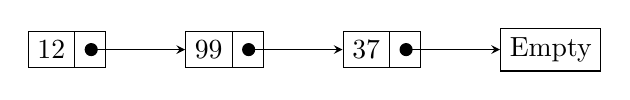
\begin{tikzpicture}[list/.style={rectangle split, rectangle split parts=2,
    draw, rectangle split horizontal}, >=stealth, start chain]

  \node[list,on chain] (A) {12};
  \node[list,on chain] (B) {99};
  \node[list,on chain] (C) {37};
  \node[on chain,draw] (D) {Empty};
  %\draw (D.north east) -- (D.south west);
  %\draw (D.north west) -- (D.south east);
  \draw[*->] let \p1 = (A.two), \p2 = (A.center) in (\x1,\y2) -- (B);
  \draw[*->] let \p1 = (B.two), \p2 = (B.center) in (\x1,\y2) -- (C);
  \draw[*->] let \p1 = (C.two), \p2 = (C.center) in (\x1,\y2) -- (D);
\end{tikzpicture}
\end{center}

\begin{itemize}
\item It is composed of a sequence of \emc{fixed size} `cells'. 
\item Each containing a \emc{head} item, and \emc{tail} pointing to the next cell.
\item The final cell points to a special cell representing the \emc{empty} list.
\end{itemize}

\begin{block}{Why focus on fixed-size cells to build dynamic data types?}
Operating systems implement allocators to provide programs with fixed areas of memory -- through costly allocations and de-allocation operations. Therefore we have to build dynamic data types (that will require more or less memory as they grow and shrink) from those units.
\end{block}
\end{frame}


\begin{frame}
\frametitle{Representing a linked list as tuples in Python.}

We will implement a linked list in Python, using \texttt{tuple} and \texttt{None}.
\begin{itemize}
\item We represent an empty linked list as the value \texttt{None}.
\item We represent a cell of a linked list as a tuple of \texttt{(head, tail)}.
\end{itemize}

\vspace{3mm}
We represent the linked list of values 12, 99 and 37 as:

\begin{center}
\texttt{(12, (99, (37, None)))}
\end{center}

\end{frame}


\begin{frame}
\frametitle{Linked list operations in Python.}

Simple algorithms on linked lists:
\begin{description}
  \item[empty()] --- returns an empty linked list (\texttt{None}).
  \item[cons(lList, item)] --- returns a list with item appended to lList.
  \item[head(lList)] --- returns the head item of the linked list.
  \item[tail(lList)] --- returns the tail linked list.
\end{description}

\vspace{3mm}
\begin{block}{Abstract interface to the linked list.}
By writing linked list algorithms to only use this restricted list of functions we can abstract the details of how linked lists are implemented. We are free to change this representation without modifying the algorithms. Such a set of functions is called an \emc{interface}.
\end{block}

\end{frame}

\begin{frame}
\frametitle{Linked list operations in Python.}

  \inputminted[
    firstline=3,
    lastline=17,
    xleftmargin=1.4em,
    frame=lines,
    framesep=2mm,
    %baselinestretch=1.2,
    % bgcolor=lightgray,
    fontsize=\footnotesize,
    linenos
  ]{python}{src/LinkedList.py}

All operations have time complexity $\mathcal{O}(1)$.


\end{frame}


\begin{frame}
\frametitle{Algorithms on linked list.}

More complex algorithms can be implemented in terms of the simpler algorithms:
\begin{description}
  \item[length(lList)] --- returns the number of items in the list.
  \item[index(lList, position)] --- returns the item at index `position' in the list, or throws an exception if it does not exist.
  \item[append(lList1, lList2)] --- returns a linked list with all elements of lList1 and lList2 in sequence.
  \item[isin(lList, item)] --- returns \texttt{True} if item is in the linked list.
  \item[Equals(lList1, lList2)] --- returns whether the lists contain exactly the same items.
\end{description}

\end{frame}

\begin{frame}
\frametitle{The length of a linked list.}

A recursive implementation to get the length of the list. Note that the equality is equivalent to a test on whether the list is empty. 

  \inputminted[
    firstline=19,
    lastline=24,
    xleftmargin=1.4em,
    frame=lines,
    framesep=2mm,
    %baselinestretch=1.2,
    % bgcolor=lightgray,
    fontsize=\footnotesize,
    linenos
  ]{python}{src/LinkedList.py}

Time complexity $\mathcal{O}(N)$ in $N$ the length of the list.

\end{frame}

\begin{frame}
\frametitle{Indexing a linked list.}

A recursive implementation of `index', to get the element position from the linked list.

  \inputminted[
    firstline=26,
    lastline=35,
    xleftmargin=1.4em,
    frame=lines,
    framesep=2mm,
    %baselinestretch=1.2,
    % bgcolor=lightgray,
    fontsize=\footnotesize,
    linenos
  ]{python}{src/LinkedList.py}

Time complexity $\mathcal{O}(N)$ in $N$ the length of the list.

\end{frame}

\begin{frame}
\frametitle{Appending two linked lists.}

A recursive implementation of appending two lists together. 

  \inputminted[
    firstline=37,
    lastline=42,
    xleftmargin=1.4em,
    frame=lines,
    framesep=2mm,
    %baselinestretch=1.2,
    % bgcolor=lightgray,
    fontsize=\footnotesize,
    linenos
  ]{python}{src/LinkedList.py}


\begin{block}{Leveraging immutability}
Note that all operations and algorithms never mutate linked lists, but instead return new ones. we leverage this in `append', to directly returns the second list once no more elements of the first one remain (line 40). If they were mutable, we would have to return a copy.
\end{block}

\end{frame}

\begin{frame}
\frametitle{Testing inclusion of an item in a linked list.}

A recursive implementation of `isin'.

  \inputminted[
    firstline=44,
    lastline=51,
    xleftmargin=1.4em,
    frame=lines,
    framesep=2mm,
    %baselinestretch=1.2,
    % bgcolor=lightgray,
    fontsize=\footnotesize,
    linenos
  ]{python}{src/LinkedList.py}

\end{frame}




\begin{frame}
\frametitle{Testing linked lists and operations.}

  \inputminted[
    firstline=53,
    lastline=68,
    xleftmargin=1.4em,
    frame=lines,
    framesep=2mm,
    %baselinestretch=1.2,
    % bgcolor=lightgray,
    fontsize=\footnotesize,
    linenos
  ]{python}{src/LinkedList.py}

\end{frame}


\begin{frame}
\frametitle{The structure of the linked list code.}

\emc{Patterns} and \emc{sources of error} in the linked list implementation:
\begin{itemize}
  \item Every operation and function takes a \emc{linked list as a first parameter}, aside from the constructor `empty'.
  \item The operation `equals' works due to the nature of the \emc{internal representation}. Those are visible to the programmer.
  \item Nothing prevents a careless programmer from passing an \emc{invalid} linked list.
  \item Validating list inputs would take $\mathcal{O}(N)$.
\end{itemize}

Could we protect the representation of the linked list, and ensure using the type system that linked lists are valid when operating on them?

\end{frame}

\section{Object Oriented Programming}

\begin{frame}
\frametitle{Objects = Data + Algorithms.}

Programming practice and style has to support a number of principles, we have explored already:

\begin{itemize}
  \item \emc{Classes}. Classes define \emc{custom types}, the \emc{operations permitted} on the type, and their  internal \emc{data representations}.
  \item \emc{Objects}. Objects are instances of a class and contain the data representing a custom type.
  \item \emc{Abstraction} \& \emc{Encapsulation}. No need to know the internal working of type to use them.
  \item \emc{Generics} \& \emc{Polymorphism}. We may use data types supporting similar operations to implement generic algorithms. 
  \item \emc{Inheritance}. Classes may inherit from others, to re-use code (do not over rely on this mechanism.)
\end{itemize}

\end{frame}


\begin{frame}
\frametitle{Classes, objects / instances and method syntax.}

  \inputminted[
    firstline=1,
    lastline=17,
    xleftmargin=1.4em,
    frame=lines,
    framesep=2mm,
    %baselinestretch=1.2,
    % bgcolor=lightgray,
    fontsize=\footnotesize,
    linenos
  ]{python}{src/toyclass.py}


\end{frame}

\begin{frame}
\frametitle{The Class LinkedList.}

  \inputminted[
    firstline=3,
    lastline=22,
    xleftmargin=1.4em,
    frame=lines,
    framesep=2mm,
    %baselinestretch=1.2,
    % bgcolor=lightgray,
    fontsize=\scriptsize,
    linenos
  ]{python}{src/LinkedListClass.py}


\end{frame}

\begin{frame}
\frametitle{Illustration of Encapsulation and Hiding.}

The implementation refactors linked list functions into a class.
\begin{itemize}
  \item Note that \texttt{\_representation} represents the internal state of the object.
  \item The underscore denotes that it should not be accessed directly as an attribute from outside the class definition.
  \item The method `cons', defined inside the class, directly manipulates this representation.
\end{itemize}

\end{frame}


\begin{frame}
\frametitle{Some algorithms as methods.}

Note we do not use the representation, even within the class.
  \inputminted[
    firstline=27,
    lastline=43,
    xleftmargin=1.4em,
    frame=lines,
    framesep=2mm,
    %baselinestretch=1.2,
    % bgcolor=lightgray,
    fontsize=\scriptsize,
    linenos
  ]{python}{src/LinkedListClass.py}


\end{frame}


\begin{frame}
\frametitle{The importance of immutability.}

We implement `append' by linking the tail of a new list to the other list directly, without first copying the other list.
  \inputminted[
    firstline=45,
    lastline=52,
    xleftmargin=1.4em,
    frame=lines,
    framesep=2mm,
    %baselinestretch=1.2,
    % bgcolor=lightgray,
    fontsize=\footnotesize,
    linenos
  ]{python}{src/LinkedListClass.py}


\end{frame}

\begin{frame}
\frametitle{Testing the LinkedList class.}

  \inputminted[
    firstline=120,
    lastline=139,
    xleftmargin=1.4em,
    frame=lines,
    framesep=2mm,
    %baselinestretch=1.2,
    % bgcolor=lightgray,
    fontsize=\scriptsize,
    linenos
  ]{python}{src/LinkedListClass.py}

\end{frame}


\begin{frame}
\frametitle{Overloading operators for seamless coding.}

How could we make our data type \texttt{LinkedList} behave like a native one?
  \inputminted[
    firstline=144,
    lastline=159,
    xleftmargin=1.4em,
    frame=lines,
    framesep=2mm,
    %baselinestretch=1.2,
    % bgcolor=lightgray,
    fontsize=\scriptsize,
    linenos
  ]{python}{src/LinkedListClass.py}


\end{frame}

\begin{frame}
\frametitle{Operators are represented by special methods.}

How could we make our data type \texttt{LinkedList} behave like a native one?
  \inputminted[
    firstline=82,
    lastline=98,
    xleftmargin=1.4em,
    frame=lines,
    framesep=2mm,
    %baselinestretch=1.2,
    % bgcolor=lightgray,
    fontsize=\scriptsize,
    linenos
  ]{python}{src/LinkedListClass.py}


\end{frame}



\begin{frame}
\frametitle{Iterators.}

Using the \texttt{yield} keyword returns the result, and `freezes' the state of the function as a \emc{generator}. Calling 'next()' continues from that point on. This allows us to implement \emc{iterators} easily:

\inputminted[
    firstline=106,
    lastline=112,
    xleftmargin=1.4em,
    frame=lines,
    framesep=2mm,
    %baselinestretch=1.2,
    % bgcolor=lightgray,
    fontsize=\scriptsize,
    linenos
  ]{python}{src/LinkedListClass.py}

Allowing the use of the object in a \texttt{for} loop:

\inputminted[
    firstline=158,
    lastline=159,
    xleftmargin=1.4em,
    frame=lines,
    framesep=2mm,
    %baselinestretch=1.2,
    % bgcolor=lightgray,
    fontsize=\scriptsize,
    linenos
  ]{python}{src/LinkedListClass.py}


\end{frame}

\section{Keeping a multi-set sorted.}

\begin{frame}
\frametitle{Motivation: keeping indexes for dynamic data structures.}

What next?
\begin{itemize}
  \item Searching is faster in sorted structures. Binary search is $\mathcal{O}(\log N)$.
  \item However, the cost of sorting is $\mathcal{O}(N \cdot \log N)$.
  \item What to do when \emc{adding or removing elements?} Sort again? No.
  \item Efficient data structures to maintain sorted sequences, and search in them
\end{itemize}

Key example: \emc{binary sorted tree}, allowing $\mathcal{O}(\cdot \log N)$ \emc{insert, remove and lookup}.


\end{frame}

\begin{frame}[fragile]
\frametitle{Trees and sorted trees.}

A tree is composed of a set of branches, each containing an \emc{item}, and a further \emc{left} and \emc{right} branch.

\begin{center}
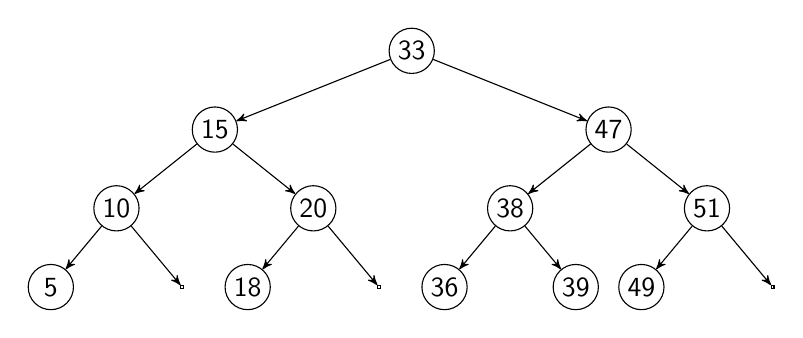
\begin{tikzpicture}[->,>=stealth',level/.style={sibling distance = 5cm/#1,
  level distance = 1cm}] 
\node [arn_n] {33}
    child{ node [arn_n] {15} 
            child{ node [arn_n] {10} 
              child{ node [arn_n] {5}} %edge from parent node[above left]
                         %{$x$}} %for a named pointer
              child{ node [arn_x] {}}
            }
            child{ node [arn_n] {20}
              child{ node [arn_n] {18}}
              child{ node [arn_x] {}}
            }                            
    }
    child{ node [arn_n] {47}
            child{ node [arn_n] {38} 
              child{ node [arn_n] {36}}
              child{ node [arn_n] {39}}
            }
            child{ node [arn_n] {51}
              child{ node [arn_n] {49}}
              child{ node [arn_x] {}}
            }
    }
; 
\end{tikzpicture}
\end{center}

\emc{Invariant} of a sorted binary tree: all items in the \emc{left branch} are \emc{smaller or equal} to the item in the branch, and all \emc{items to the right larger}.

\end{frame}

\begin{frame}
\frametitle{Representing a branch as a Python class.}

Each branch is an instance of a class, containing 3 attributes. 
\inputminted[
    firstline=1,
    lastline=11,
    xleftmargin=1.4em,
    frame=lines,
    framesep=2mm,
    %baselinestretch=1.2,
    % bgcolor=lightgray,
    fontsize=\scriptsize,
    linenos
  ]{python}{src/binaryTree.py}
By convention we represent an empty branch as \texttt{None}. The \texttt{\_\_slots\_\_} class variable pre-declares the only attributes for a more efficient representation.

\end{frame}

\begin{frame}[fragile]
\frametitle{How to add an element to the Tree.}

How to insert the item 25 to the tree?

\begin{center}
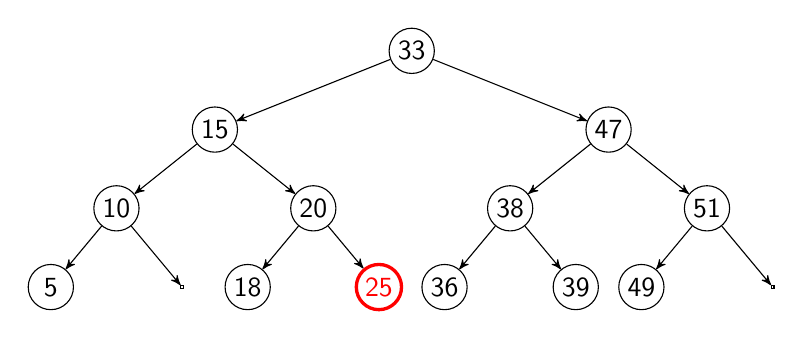
\begin{tikzpicture}[->,>=stealth',level/.style={sibling distance = 5cm/#1,
  level distance = 1cm}] 
\node [arn_n] {33}
    child{ node [arn_n] {15} 
            child{ node [arn_n] {10} 
              child{ node [arn_n] {5}} %edge from parent node[above left]
                         %{$x$}} %for a named pointer
              child{ node [arn_x] {}}
            }
            child{ node [arn_n] {20}
              child{ node [arn_n] {18}}
              child{ node [arn_r] {25}}
            }                            
    }
    child{ node [arn_n] {47}
            child{ node [arn_n] {38} 
              child{ node [arn_n] {36}}
              child{ node [arn_n] {39}}
            }
            child{ node [arn_n] {51}
              child{ node [arn_n] {49}}
              child{ node [arn_x] {}}
            }
    }
; 
\end{tikzpicture}
\end{center}
Navigate from the root of the tree to the position where the item should be inserted, at a leaf, and place a new branch there with the item.

\end{frame}

\begin{frame}
\frametitle{Adding items.}

Follow the correct left or right branch according to the invariant. When it finds the first empty leaf (\texttt{None}) insert a new branch with the item.
\inputminted[
    firstline=13,
    lastline=24,
    xleftmargin=1.4em,
    frame=lines,
    framesep=2mm,
    %baselinestretch=1.2,
    % bgcolor=lightgray,
    fontsize=\footnotesize,
    linenos
  ]{python}{src/binaryTree.py}
Note the use of recursion; and the mutation of the tree.

\end{frame}

\begin{frame}
\frametitle{Finding items.}

A recursive \emc{divide-and-conquer} algorithm for finding an element.
\inputminted[
    firstline=26,
    lastline=36,
    xleftmargin=1.4em,
    frame=lines,
    framesep=2mm,
    %baselinestretch=1.2,
    % bgcolor=lightgray,
    fontsize=\footnotesize,
    linenos
  ]{python}{src/binaryTree.py}

Key question: What does it mean to find an element? Is the element not simply going to be equal to the item passed to the \texttt{get} method? 
\end{frame}

\begin{frame}
\frametitle{Implementing `isin' using `get'.}

We note that \texttt{None} is returned when the element is now found.
\inputminted[
    firstline=38,
    lastline=40,
    xleftmargin=1.4em,
    frame=lines,
    framesep=2mm,
    %baselinestretch=1.2,
    % bgcolor=lightgray,
    fontsize=\footnotesize,
    linenos
  ]{python}{src/binaryTree.py}

\vspace{3mm}
Note that an Exception could be thrown and caught instead, to avoid reliance on checking the returned result for \texttt{None}, and also to be able to store \texttt{None} in the tree.

\end{frame}

\begin{frame}[fragile]
\frametitle{Removing items --- Case 1: removing a leaf.}

When removing a leaf (branch with no branches, eg.\ 49) we can simply replace it with \texttt{None}.
\begin{center}
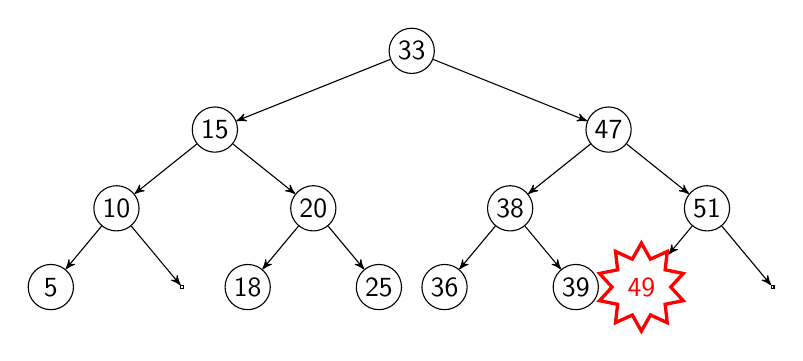
\begin{tikzpicture}[->,>=stealth',level/.style={sibling distance = 5cm/#1,
  level distance = 1cm}] 
\node [arn_n] {33}
    child{ node [arn_n] {15} 
            child{ node [arn_n] {10} 
              child{ node [arn_n] {5}} %edge from parent node[above left]
                         %{$x$}} %for a named pointer
              child{ node [arn_x] {}}
            }
            child{ node [arn_n] {20}
              child{ node [arn_n] {18}}
              child{ node [arn_n] {25}}
            }                            
    }
    child{ node [arn_n] {47}
            child{ node [arn_n] {38} 
              child{ node [arn_n] {36}}
              child{ node [arn_n] {39}}
            }
            child{ node [arn_n] {51}
              child{ node [arn_d] {49}}
              child{ node [arn_x] {}}
            }
    }
; 
\end{tikzpicture}
\end{center}
In the trivial case where the item to be removed does not have both branches, it can simply be removed, and the tree patched.

\end{frame}

\begin{frame}[fragile]
\frametitle{Case 2 \& 3: remove an incomplete branch.}

When one of the branches is \texttt{None} (eg.\ 51), we can simply `promote up' the single existing branch.
\begin{center}
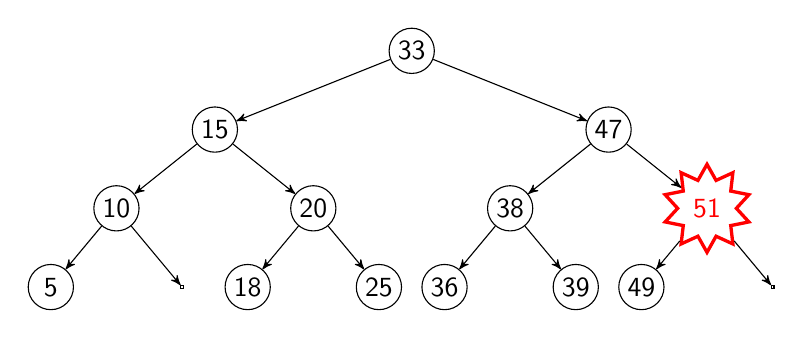
\begin{tikzpicture}[->,>=stealth',level/.style={sibling distance = 5cm/#1,
  level distance = 1cm}] 
\node [arn_n] {33}
    child{ node [arn_n] {15} 
            child{ node [arn_n] {10} 
              child{ node [arn_n] {5}} %edge from parent node[above left]
                         %{$x$}} %for a named pointer
              child{ node [arn_x] {}}
            }
            child{ node [arn_n] {20}
              child{ node [arn_n] {18}}
              child{ node [arn_n] {25}}
            }                            
    }
    child{ node [arn_n] {47}
            child{ node [arn_n] {38} 
              child{ node [arn_n] {36}}
              child{ node [arn_n] {39}}
            }
            child{ node [arn_d] {51}
              child{ node [arn_n] {49}}
              child{ node [arn_x] {}}
            }
    }
; 
\end{tikzpicture}
\end{center}
In the trivial case where the item to be removed does not have both branches, it can simply be removed, and the tree patched.

\end{frame}



\begin{frame}[fragile]
\frametitle{Case 4: a full branch}

Removing items (eg.\ 47) leaves a `hole' in the tree, and we need to substitute the item with another value. Note that we can substitute in the largest value in the left subtree (eg.\ 39).

\begin{center}
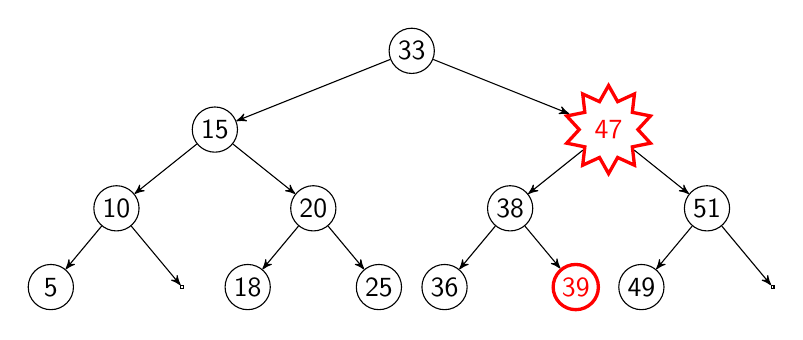
\begin{tikzpicture}[->,>=stealth',level/.style={sibling distance = 5cm/#1,
  level distance = 1cm}] 
\node [arn_n] {33}
    child{ node [arn_n] {15} 
            child{ node [arn_n] {10} 
              child{ node [arn_n] {5}} %edge from parent node[above left]
                         %{$x$}} %for a named pointer
              child{ node [arn_x] {}}
            }
            child{ node [arn_n] {20}
              child{ node [arn_n] {18}}
              child{ node [arn_n] {25}}
            }                            
    }
    child{ node [arn_d] {47}
            child{ node [arn_n] {38} 
              child{ node [arn_n] {36}}
              child{ node [arn_r] {39}}
            }
            child{ node [arn_n] {51}
              child{ node [arn_n] {49}}
              child{ node [arn_x] {}}
            }
    }
; 
\end{tikzpicture}
\end{center}
In the trivial case where the item to be removed does not have both branches, it can simply be removed, and the tree patched.

\end{frame}

\begin{frame}
\frametitle{The remove Python implementation.}

\inputminted[
    firstline=69,
    lastline=89,
    xleftmargin=1.4em,
    frame=lines,
    framesep=2mm,
    %baselinestretch=1.2,
    % bgcolor=lightgray,
    fontsize=\scriptsize,
    linenos
  ]{python}{src/binaryTree.py}


\end{frame}

\begin{frame}
\frametitle{Traversing in order: Depth-first traversal}

Depth-first traversal involves returning items, by first returning all nodes in the left branch, then the item, and all items in the right branch. Due to the sorted tree invariants, items are returned in order.

\inputminted[
    firstline=91,
    lastline=97,
    xleftmargin=1.4em,
    frame=lines,
    framesep=2mm,
    %baselinestretch=1.2,
    % bgcolor=lightgray,
    fontsize=\scriptsize,
    linenos
  ]{python}{src/binaryTree.py}

This is the second example of a \emc{generator} defined through the keyword \texttt{yield}. The keyword \texttt{yield from} returns items from another generator until its is \emc{exhausted}, then continues the execution. More here: \url{https://wiki.python.org/moin/Generators}.

\end{frame}

\begin{frame}
\frametitle{Testing add and remove}

We test at the level of the interface, not internal representation.
\inputminted[
    firstline=124,
    lastline=139,
    xleftmargin=1.4em,
    frame=lines,
    framesep=2mm,
    %baselinestretch=1.2,
    % bgcolor=lightgray,
    fontsize=\scriptsize,
    linenos
  ]{python}{src/binaryTree.py}

The \texttt{enumerate} function takes a sequence and returns an iterator of tuples, of the position and each element in order.

\end{frame}

\begin{frame}
\frametitle{Testing the iterator}

We ensure that iterating returns elements in order.
\inputminted[
    firstline=141,
    lastline=153,
    xleftmargin=1.4em,
    frame=lines,
    framesep=2mm,
    %baselinestretch=1.2,
    % bgcolor=lightgray,
    fontsize=\scriptsize,
    linenos
  ]{python}{src/binaryTree.py}

The \texttt{zip} function takes two iterators or sequences, and returns tuples with an element from each.

\end{frame}


\begin{frame}
\frametitle{Computational complexity.}

Average case operation:
\begin{itemize}
  \item \emc{add}, \emc{remove}, \emc{get}, \emc{isin}: $\mathcal{O}(\log N)$
  \item \emc{walk}, \emc{len}, \emc{depth} walk the full tree: $\mathcal{O}(N)$
\end{itemize}
Note that \texttt{branch} is mutable -- and the associated risks.

\vspace{3mm}
\begin{block}{Advanced data structures: Balanced trees}
The average case performance is only attained if the tree is `balanced'. However trees might get unbalanced under dynamic additions and deletions (consider adding elements in order). Balanced binary trees are needed to ensure balance is maintained for $\mathcal{O}(\log N)$ operations.
\end{block}

\end{frame}

\section{Mapping types \& the Python \texttt{dict} type.}

\begin{frame}
\frametitle{From binary sorted trees to mapping types.}

\begin{itemize}
  \item We presented a \emc{container} for items: it stores a \emc{dynamically sized sequence sorted}, and also to \emc{quickly lookup} items.
  \item However we want to implement an \emc{efficient key-value} store.
\end{itemize}

\inputminted[
    firstline=107,
    lastline=114,
    xleftmargin=1.4em,
    frame=lines,
    framesep=2mm,
    %baselinestretch=1.2,
    % bgcolor=lightgray,
    fontsize=\scriptsize,
    linenos
  ]{python}{src/minimap.py}

Can we build \texttt{minimap} this from the \texttt{branch} data type?
\end{frame}

\begin{frame}
\frametitle{Items stored in the tree can be custom data types.}

There is no reason to limit the items stored in \texttt{branch} to simple Python data types. Any custom type that defines equals, less than, and less or equal may be used -- through the wonder of generic programming.

\vspace{3mm}
We define a custom data type \texttt{KeyValue} representing a key-value pair, with a mutable value:
\inputminted[
    firstline=3,
    lastline=12,
    xleftmargin=1.4em,
    frame=lines,
    framesep=2mm,
    %baselinestretch=1.2,
    % bgcolor=lightgray,
    fontsize=\scriptsize,
    linenos
  ]{python}{src/minimap.py}

\end{frame}

\begin{frame}
\frametitle{Define equality and less than operator for \texttt{KeyValue}.}

We define the custom operators for key-values so that they can be used within the tree.
\inputminted[
    firstline=14,
    lastline=21,
    xleftmargin=1.4em,
    frame=lines,
    framesep=2mm,
    %baselinestretch=1.2,
    % bgcolor=lightgray,
    fontsize=\scriptsize,
    linenos
  ]{python}{src/minimap.py}

Note that ordering operations and equality are only defines on the keys, not the values. Instances with the same key form an equivalence set.

\end{frame}


\begin{frame}
\frametitle{Define the minimap type \& insertion operation.}

\inputminted[
    firstline=24,
    lastline=42,
    xleftmargin=1.4em,
    frame=lines,
    framesep=2mm,
    %baselinestretch=1.2,
    % bgcolor=lightgray,
    fontsize=\scriptsize,
    linenos
  ]{python}{src/minimap.py}

\end{frame}



\begin{frame}
\frametitle{The indexing operator to retrieve values by key.}

Construct a generic \texttt{KeyValue} item based on a key, and use `get' to get the matching item.
\inputminted[
    firstline=44,
    lastline=54,
    xleftmargin=1.4em,
    frame=lines,
    framesep=2mm,
    %baselinestretch=1.2,
    % bgcolor=lightgray,
    fontsize=\scriptsize,
    linenos
  ]{python}{src/minimap.py}

\end{frame}

\begin{frame}
\frametitle{Testing minimap get and set.}

Define a fixture with a minimap and a couple of lists.
\inputminted[
    firstline=100,
    lastline=105,
    xleftmargin=1.4em,
    frame=lines,
    framesep=2mm,
    %baselinestretch=1.2,
    % bgcolor=lightgray,
    fontsize=\scriptsize,
    linenos
  ]{python}{src/minimap.py}

Set and get all items from the fixture.
\inputminted[
    firstline=123,
    lastline=130,
    xleftmargin=1.4em,
    frame=lines,
    framesep=2mm,
    %baselinestretch=1.2,
    % bgcolor=lightgray,
    fontsize=\scriptsize,
    linenos
  ]{python}{src/minimap.py}

\end{frame}

\begin{frame}
\frametitle{The builtin \texttt{dict} type.}

The Python dictionary type provides a very efficient key-value store.
\begin{itemize}
  \item the \texttt{dict} function takes a sequence of tuples and returns a dictionary mapping them as key values.
  \item There is a shorthand for dict literals, eg. \texttt{\{k1:v1, k2:v2\}}
  \item Get and set operations are as in minimap, eg. \texttt{m[k] = v} for set, and \texttt{m[k]} for get.
  \item the \texttt{len} function returns the number of items, and an iterator returns an unordered sequence of keys.
\end{itemize}

\vspace{3mm} 
For a full list of operations see \url{https://docs.python.org/3.6/library/stdtypes.html\#mapping-types-dict}.

\end{frame}

\section{From programming to learning.}

\begin{frame}

\frametitle{The machine learning paradigm}

\begin{itemize}
  \item Some problems do not have a \emc{suitable logical structure} to easily program an algorithm to solve them.
  \item Usually they deal with \emc{raw unstructured data}: natural language, images, raw sensor inputs, etc. 
  \item Humans are very good at some of them. Eg. recognizing faces, understanding language, classifying cats versus dogs in pictures.
  \item But humans are very bad at understanding why, and how they make those decisions.
\end{itemize}

\vspace{3mm}
Machine learning algorithms instead learn by example from a training set, and can then perform the task required.

\end{frame}

\begin{frame}

\frametitle{Sample task: recognizing French vs. German fragments of text}

Problem statement: I give you a fragment of 200 characters of text. Is it in French or in German?

\begin{itemize}
  \item Approach 1 --- Expert system: \emc{employ expert linguists} to tell you all, or the best ways, to differentiate the two languages in a small fragment.
  \item Approach 2 --- Machine learning: use a set of known French and German fragment to \emc{train a model to differentiate} between the languages.
\end{itemize}

\vspace{3mm}
The model we consider here is a \emc{Random Decision Forrest}, which is a collection of \emc{Decision Trees} -- linking to our current material.

\end{frame}

\begin{frame}[fragile]

\frametitle{Decision Trees.}

Branches contain a \emc{weak classifier}, eg.\ whether the item to be classified \emc{contains a specific substring}, branching left (`yes') or right (`no'). Leafs contain \emc{classification decisions}.

\begin{center}
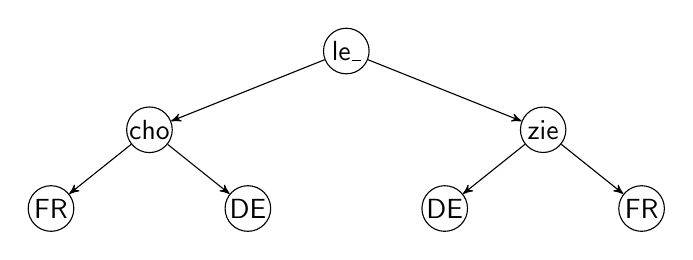
\begin{tikzpicture}[->,>=stealth',level/.style={sibling distance = 5cm/#1,
  level distance = 1cm}] 
\node [arn_n] {le\_} 
            child{ node [arn_n] {cho} 
              child{ node [arn_n] {FR}} %edge from parent node[above left]
                         %{$x$}} %for a named pointer
              child{ node [arn_n] {DE}}
            }
            child{ node [arn_n] {zie}
              child{ node [arn_n] {DE}}
              child{ node [arn_n] {FR}}
            }                            
; 
\end{tikzpicture}
\end{center}

To classify an item, follow the path to a decision leaf.

\end{frame}

\begin{frame}

\frametitle{Training Decision Trees.}

Given: a training set of text fragment with known language labels.
\begin{itemize}
  \item Start with a 1 branch tree: select a number of random features, and pick the one that separates the two classes best.
  \item Separate items left and right, according to the selected feature.
  \item Recursively, train the left and right branch until a maximum depth.
\end{itemize}

\vspace{3mm}
What is the criterium to select the best feature: the one that minimizes the \emc{mean Gini impurity}:
$gini = 1 - p_0^2 - p_1^2$,
where $p_0$ and $p_1$ are the fraction of items belonging to each class.

\end{frame}

\begin{frame}
\frametitle{Preparing training and evaluation datasets (1).}

\inputminted[
    firstline=87,
    lastline=102,
    xleftmargin=1.4em,
    frame=lines,
    framesep=2mm,
    %baselinestretch=1.2,
    % bgcolor=lightgray,
    fontsize=\scriptsize,
    linenos
  ]{python}{src/randomforest.py}

\end{frame}

\begin{frame}
\frametitle{Preparing training and evaluation datasets (2).}

\inputminted[
    firstline=104,
    lastline=113,
    xleftmargin=1.4em,
    frame=lines,
    framesep=2mm,
    %baselinestretch=1.2,
    % bgcolor=lightgray,
    fontsize=\scriptsize,
    linenos
  ]{python}{src/randomforest.py}

Note that the format of each item to be trained on or be evaluated is (label, feature set, original item). The variable features gathers all features in the training set, ie.\ all substrings of length 3.

\end{frame}

\begin{frame}
\frametitle{The decision tree class.}

\inputminted[
    firstline=39,
    lastline=47,
    xleftmargin=1.4em,
    frame=lines,
    framesep=2mm,
    %baselinestretch=1.2,
    % bgcolor=lightgray,
    fontsize=\scriptsize,
    linenos
  ]{python}{src/randomforest.py}

An instance may be either a branch (if feature is not None) including a feature and a left and right decision tree; or a final binary decision.

\end{frame}

\begin{frame}
\frametitle{Training a decision tree.}

\inputminted[
    firstline=49,
    lastline=66,
    xleftmargin=1.4em,
    frame=lines,
    framesep=2mm,
    %baselinestretch=1.2,
    % bgcolor=lightgray,
    fontsize=\scriptsize,
    linenos
  ]{python}{src/randomforest.py}

Steps represents the number of features tried per branch.
\end{frame}


\begin{frame}
\frametitle{Measuring impurity for a candidate feature.}

\inputminted[
    firstline=19,
    lastline=35,
    xleftmargin=1.4em,
    frame=lines,
    framesep=2mm,
    %baselinestretch=1.2,
    % bgcolor=lightgray,
    fontsize=\scriptsize,
    linenos
  ]{python}{src/randomforest.py}

The gini function computes the gini coefficient on the items' labels.
\end{frame}


\begin{frame}
\frametitle{Classification using a decision tree.}

\inputminted[
    firstline=68,
    lastline=80,
    xleftmargin=1.4em,
    frame=lines,
    framesep=2mm,
    %baselinestretch=1.2,
    % bgcolor=lightgray,
    fontsize=\scriptsize,
    linenos
  ]{python}{src/randomforest.py}

Decision leafs store the most likely 0 or 1 label. Classification routes the item given the the leaf according to all intermediate features.
\end{frame}

\begin{frame}
\frametitle{The evaluation of machine learning systems.}

\begin{itemize}
  \item You must evaluate the accuracy, true positive and false positive rate for classifiers.
  \item Train and evaluate on a separate subset of labeled data.
  \item Accuracy: the fraction of correct decisions.
  \item Key visualization for TP/FP: the ROC curve.
\end{itemize}

\end{frame}

\begin{frame}
\frametitle{Evaluation pipeline, using a Random Forest.}

\inputminted[
    firstline=115,
    lastline=133,
    xleftmargin=1.4em,
    frame=lines,
    framesep=2mm,
    %baselinestretch=1.2,
    % bgcolor=lightgray,
    fontsize=\scriptsize,
    linenos
  ]{python}{src/randomforest.py}

\end{frame}

\begin{frame}
\frametitle{Results setup}

Setup:
\begin{itemize}
  \item Use `Faust' for DE and `The Mysterious island' for FR.
  \item Extract fragments of 200 characters.
  \item Train using 400 fragments for each language.
  \item Test 100 random features per branch for training.
  \item Evaluate with 200 fragments for each language.
\end{itemize}

For a single tree of level 1 depth, accuracy is about 50\%--60\%. That is pretty poor -- and close to random guessing.

\end{frame}


\begin{frame}
\frametitle{Results for 40 decision trees}

Accuracy: over 98\%.

\vspace{3mm}
Where are the errors? 
\begin{itemize}
  \item ``The text strictly follows the original. Corrections made in later print editions have been denoted in square brackets. \ldots''
  \item ``is agreement violates the law of the state applicable to this agreement, the agreement shall be interpreted to make the maximum \ldots''
  \item \ldots
\end{itemize}

These are fragments of neither FR or DE text! Lesson: \emc{compare the performance of ML systems with the performance of humans}, not just ground truth!

\end{frame}

\begin{frame}
\frametitle{True / False positive rates}

As an ML system designer you can tune your classifier. However, any tuning leads to a trade off between the \emc{True Positive Rate} (TPR) and the \emc{False Positive Rate} (FPR).

\begin{itemize}
  \item \emc{True Positive Rate}: The number of items that are positive, classified as positive.
  \item \emc{False Positive Rate}: The number of items that are negative, classified as positive.
\end{itemize}

\vspace{3mm}
The trade-off between TPR / FPR is captured in the ROC curve visualization.

\end{frame}

\begin{frame}
\frametitle{Receiver Operating Characteristic Curves}

\begin{center}
\includegraphics[scale=0.5]{assets/ROC}
\end{center}

\end{frame}


\begin{frame}
\frametitle{ More on Machine Learning \ldots }

Great tutorial on Random Decision Forests:
\begin{itemize}
  \item Criminisi, A., Shotton, J., \& Konukoglu, E. (2011). Decision forests for classification, regression, density estimation, manifold learning and semi-supervised learning. Microsoft Research Cambridge, Tech. Rep. MSRTR-2011-114, 5(6), 12.
  \item Fundamentals of Deep Learning by Nikhil Buduma and Nicholas Lacascio. O'Reilly, June 2017.
\end{itemize}

\vspace{3mm}
You may find some of those on-line.
\end{frame}


\section{Ethics, Machine Learning and Artificial Intelligence.}

\begin{frame}
\frametitle{ Ethical issues around machine learning }

\begin{itemize}
  \item Privacy concerns, related to training and classification.
  \item Understandability of classification -- and the difficulty of explaining why a decision was reached.
  \item Issues around algorithmic discrimination.
  \item Liability and responsibility: who is to blame if ML systems take the wrong decision, or take a wrong action.
  \item Potential for ethical reasoning, and harm.
  \item Autonomous weapons and warfare.
\end{itemize}

\end{frame}

\section{Exercises.}

\begin{frame}

\frametitle{Exercise 3-1. Refactor out recursion from \texttt{LinkedList}.}

\begin{description}
  \item[3-1.1] Try to use the LinkedList class to store a list of may items, and successively compute its length. What happens?
  \item[3-1.2] Refactor each method of LinkedList to remove recursion, and test your work through suitable tests.
  \item[3-1.3] Why is it appropriate to use recursion to implement methods in branch, but not in the LinkedList class?
\end{description}

\end{frame}


\begin{frame}

\frametitle{Exercise 3-2. Improve trees.}

\begin{description}
  \item[3-2.1] Implement the length method on \texttt{branch} to gives the number of items stored in the tree.
  \item[3-2.2] Implement the depth method, that returns the maximum depth of the tree, namely the highest number of branches any item is from the root.
  \item[3-3.3] Justify the time complexity of those operations.
\end{description}


\end{frame}

\begin{frame}

\frametitle{Exercise 3-3. Improve \texttt{minimap}.}

\begin{description}
  \item[3-3.1] Implement the \texttt{\_\_delitems\_\_} operation on \texttt{minimap} allowing library users to delete keys via \texttt{del M[k]}.
  \item[3-3.2] Implement the \texttt{\_\_contains\_\_} operation that tests whether a key is within the key-value store.
  \item[3-3.3] Implement an iterator on the minimap that iterates over all keys in sorted order. (Hint: understand how to use generators.)
  \item[3-3.4] Implement a separate iterator \texttt{iteritems} returning a sequence of the key value pairs contained in the minimap.
\end{description}

\end{frame}

\begin{frame}

\frametitle{Exercise 3-4. Understand \texttt{dict} and friends.}

\begin{description}
  \item[3-4.1] Write a program using a \texttt{dict} variable, that reads over a file, and produces a count of the number of times each word was seen. Write a tally to a file.
  \item[3-4.2] Study the \texttt{collections} standard library and the \texttt{defaultdict} and \texttt{OrderedDict} types. Refactor your code to use whichever may be appropriate.
  \item[3-4.3] Study the \texttt{Counter} type from \texttt{collections} and refactor once more your code to use it. 
  \item[3-4.3] Implement a \texttt{Counter} data type using a \texttt{dict} datatype, and no types from collections.
\end{description}

\end{frame}

\begin{frame}

\frametitle{Exercise 3-5. From languages to styles.}

The Random Decision Forest example distinguishes between languages. Adapt the algorithm, to attempt to distinguish between fragments from two novels written in English by different authors. Report on the performance of your classifier using standard evaluation measures for fragments of different lengths.

\end{frame}


% ---------------------------------

\bibliographystyle{alpha}
\nobibliography{references}

\end{document}